\section{Laparoscopic tool manipulation}

The biggest challenge in manipulating a laparoscopic tool with a robot is overcoming the \textbf{fulcrum effect} problem. This is also one of the reasons that 
robotic assisted surgery replaced the traditional laparoscopic procedures. The fulcrum effect means that the surgeon's hand motions are inverted and scaled 
with respect to the Remote Center of Motion point, which lies approximately on the center of the incision. Apart from the scaling and inversion, laparoscopic 
procedures add an additional motion constraint that demands at each time one point of the laparoscopic tool to coincide with the RCM point.

\subsection{Tool pose}

\begin{center}
\begin{figure}[H]
\centering
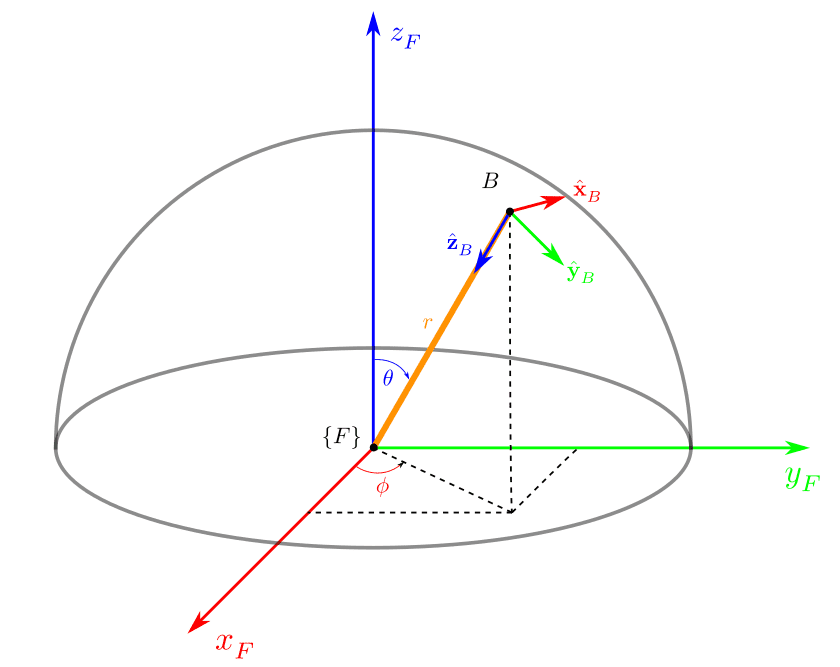
\includegraphics[width=12cm]{images/fulcrum-space.png}\\
\caption{Tool pose at target point $B$ calculated with respect to Fulcrum's reference frame $\lbrace F \rbrace$}
\end{figure}
\end{center}

The laparoscopic tool pose is given by the position and orientation vectors at target point $B$ with respect to the coordinate frame $\lbrace F \rbrace$.
The pose is given by the following transformation matrix
\[
{}^{F}T_B = \begin{bmatrix}
{}^{F}R_B & {}^{F}\mathbf{p}^{}_B \\
\mathbf{0} & 1 \\
\end{bmatrix}
\;\; where \;\;
{}^{F}R_B = \begin{bmatrix}
\hat{\mathbf{x}}^{}_B & \hat{\mathbf{y}}^{}_B & \hat{\mathbf{z}}^{}_B \\
\end{bmatrix}
\]

\[
\hat{\mathbf{x}}^{}_B = \hat{\mathbf{θ}} = cos(θ)cos(φ)\hat{\mathbf{x}}^{}_F + cos(θ)sin(φ)\hat{\mathbf{y}}^{}_F - sin(θ)\hat{\mathbf{z}}^{}_F
= \begin{bmatrix}
cos(θ)cos(φ) \\
cos(θ)sin(φ) \\
- sin(θ) \\
\end{bmatrix}
\]

\[
\hat{\mathbf{y}}^{}_B = \hat{\mathbf{φ}} = -sin(φ)\hat{\mathbf{x}}^{}_F + cos(φ)\hat{\mathbf{y}}^{}_F
= \begin{bmatrix}
-sin(φ) \\
cos(φ) \\
0 \\
\end{bmatrix}
\]

\[
\hat{\mathbf{z}}^{}_B = - \hat{\mathbf{r}} = - (sin(θ)cos(φ)\hat{\mathbf{x}}^{}_F + sin(θ)sin(φ)\hat{\mathbf{y}}^{}_F + cos(θ)\hat{\mathbf{z}}^{}_F)
= \begin{bmatrix}
-sin(θ)cos(φ) \\
-sin(θ)sin(φ) \\
-cos(θ) \\
\end{bmatrix}
\]

The position of the point $B$ is given in spherical coordinates by:
\begin{itemize}
	\item $r=ρ$ : outside penetration of laparoscopic tool
	\item $θ=β$ : altitude angle
	\item $φ=α$ : orientation angle
\end{itemize}
thus the position with respect to the coordinate frame $\lbrace F \rbrace$ is given by
\[
{}^{F}\mathbf{p}^{}_B = \begin{bmatrix}
ρsin(β)cos(α) \\
ρsin(β)sin(α) \\
ρcos(β) \\
\end{bmatrix} = ρ \hat{\mathbf{r}}
\]

The above goal point must be the same as the $TCP$ point of the robot's end-effector. This means, that this pose must be converted with respect to the robot's reference frames.
\[
{}^{U}T^{}_{TCP} = {}^{U}T^{}_{B}
\]
\[
{}^{U}T^{}_{0} \; {}^{0}T^{}_{7} \; {}^{7}T^{}_{TCP} = {}^{U}T^{}_{F} \; {}^{F}T^{}_{B}
\]
\begin{equation}
{}^{0}T^{}_{7} = {}^{U}T^{-1}_{0} \; {}^{U}T^{}_{F} \; {}^{F}T^{}_{B} \; {}^{7}T^{-1}_{TCP}
\end{equation}

\subsection{Pivoting motion with respect to Fulcrum Point}
\label{subsection:pivot-motions}

On this section, some basic pivoting trajectories around the fulcrum point, are presented. In all of the following three example pivoting motions, we have made 
the assumption that the position and orientation of the ${F}$ reference frame is precisely known, which is however not applicable in real-life scenarios ()

\subsubsection{Circular trajectory of tool tip}

\begin{center}
\begin{figure}[H]
\centering
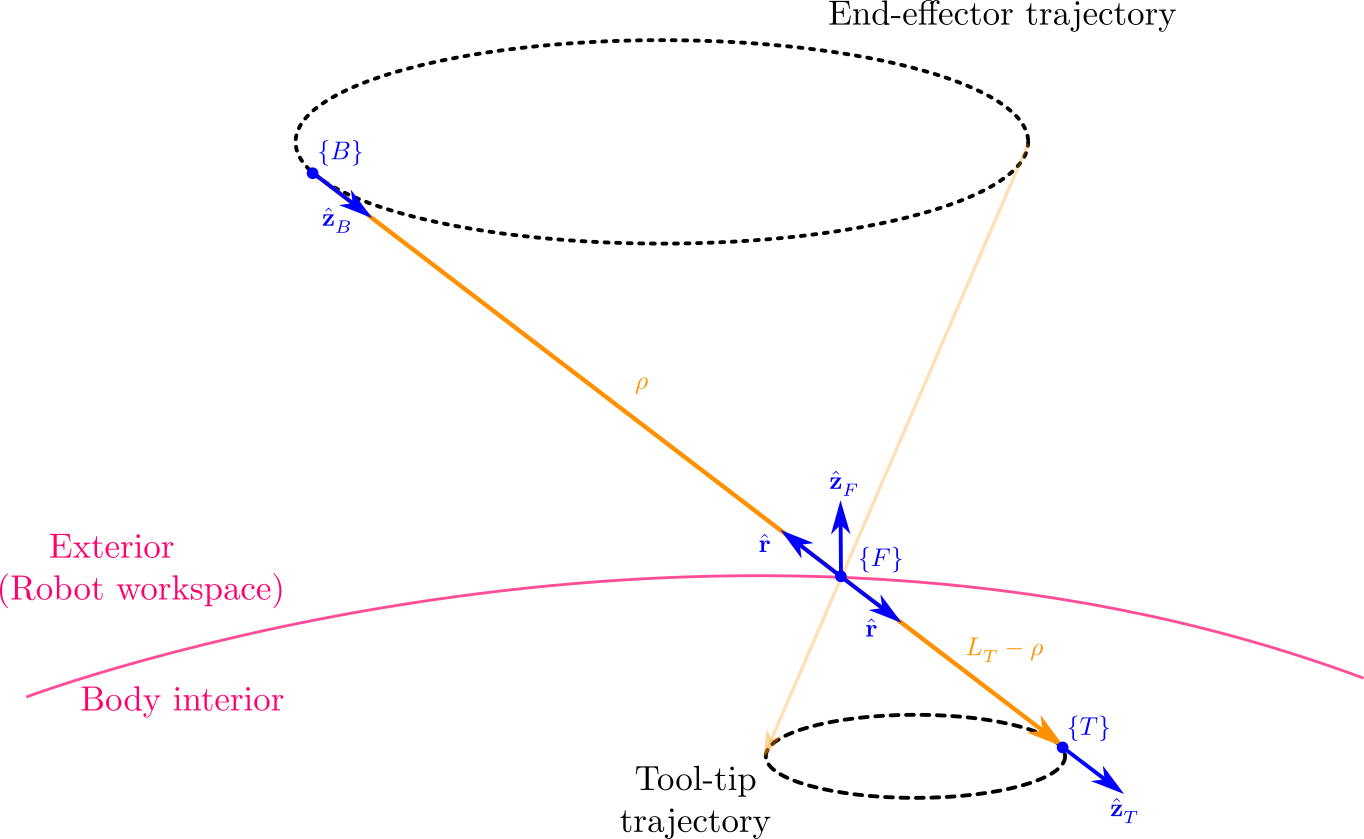
\includegraphics[width=12cm]{images/circular-trajectory-wrt-fulcrum.png}\\
\caption{Circular trajectory of tool tip with respect to Fulcrum reference frame}
\end{figure}
\end{center}

To generate a circular trajectory for the pivot movement we must specify the center of the circle 
and a vector whose magnitude is the radius of the circle and it’s direction gives the orientation 
of the plane that the circle lies at. The simplest case of a circular trajectory is the one, 
whose circle lies in a plane parallel to the xy plane.


We first consider the motion of the laparoscopic tool tip on a circle parallel to a z-plane, with respect to the $\lbrace F \rbrace$ coordinate frame.
\[
(x^{}_{F} - x^{}_{F0})^2 + (y^{}_{F} - y^{}_{F0})^2 = r_0^2, \;\; z^{}_{F} = z^{}_{F0}
\]
It's often more convenient to express trajectories in a parametric form, which makes it easier to calculate all the waypoints of the trajectory
\[
\begin{cases}
x^{}_{F} = r_0cos(2πt) + x^{}_{F0} \\
y^{}_{F} = r_0sin(2πt) + y^{}_{F0} \\
z^{}_{F} = z^{}_{F0}
\end{cases} ,
\;\;
t \in [0, 1]
\]
After having calculated the cartesian coordinates we can calculate the spherical coordinates as follows
\begin{equation}
\label{eqns:cartesian-to-spherical}
\begin{cases}
r = \sqrt{x^{2}_{F} + y^{2}_{F} + z^{2}_{F}} \\
θ = atan2 \left( \sqrt{x^{2}_{F} + y^{2}_{F}}, z^{}_{F} \right) \\
φ = atan2(y^{}_{F}, x^{}_{F})
\end{cases}
\end{equation}

\subsubsection{Circular arc trajectory of tool tip}

To generate a circular arc trajectory for a pivot motion we must specify the same parameters as 
in the circular trajectory as well as the length of the arc or the total angle of the arc 
section.


\subsubsection{Line segment trajectory of tool tip}

\begin{center}
\begin{figure}[H]
\centering
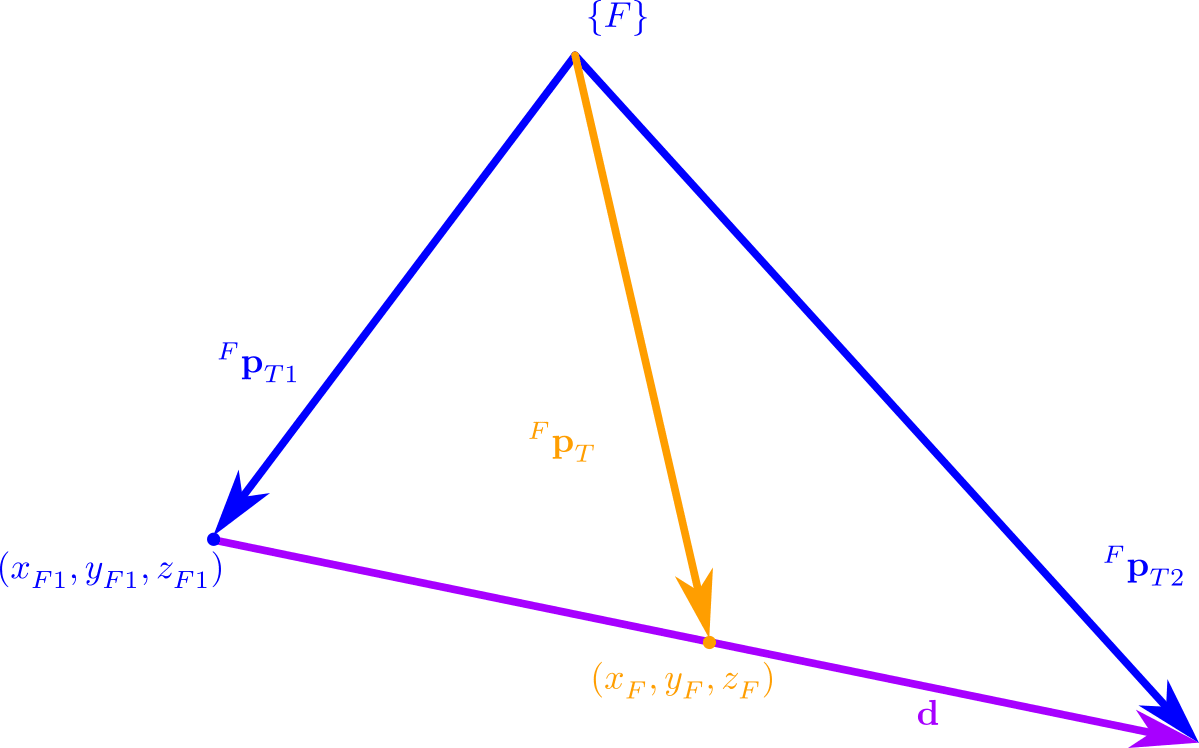
\includegraphics[width=10cm]{images/line-segment-trajectory-wrt-fulcrum.png}\\
\caption{Line segment trajectory of tool tip with respect to Fulcrum reference frame}
\end{figure}
\end{center}
\[
\mathbf{d} = {}^{F}\mathbf{p}^{}_{T2} - {}^{F}\mathbf{p}^{}_{T1} = [l, m, n]^\top
\]
\[
{}^{F}\mathbf{p}^{}_{T} = [x^{}_{F}, y^{}_{F}, z^{}_{F}]^\top
\]
\[
{}^{F}\mathbf{p}^{}_{T} = {}^{F}\mathbf{p}^{}_{T1} + t\mathbf{d}
\]
\[
t = \frac{x^{}_{F} - x^{}_{F1}}{l} = \frac{y^{}_{F} - y^{}_{F1}}{m} = \frac{z^{}_{F} - z^{}_{F1}}{n} \;\; t \in [0, 1]
\]
\[
\begin{cases}
x^{}_{F} = tl + x^{}_{F1} = (1-t)x^{}_{F1} + tx^{}_{F2} \\
y^{}_{F} = tm + y^{}_{F1} = (1-t)y^{}_{F1} + ty^{}_{F2} \\
z^{}_{F} = tn + z^{}_{F1} = (1-t)z^{}_{F1} + tz^{}_{F2}
\end{cases}
\]
After having calculated the cartesian coordinates we can calculate the spherical coordinates using the \ref{eqns:cartesian-to-spherical} equations.

The line segment trajectory of tool tip, as analysed in this section needs no implementation as 
it is already implemented in the ROS MoveIt library and can be used by calling the method 
\textbf{computeCartesianPath}.

\subsection{Task space analysis}

Dexterity analysis for tool's task space
\begin{equation}
\mathcal{D} = \mathcal{L}_q \mathcal{M}
\end{equation}
where
\begin{equation}
\mathcal{M} = \sqrt{det(J J^\top)}
\end{equation}
\begin{equation}
\label{dexterity-measure}
\mathcal{L}_{q}=1-\exp\left\{-\kappa\prod_{i=1}^{n_{k}}\frac{(q_{ {i}}-q_{i,\min})(q_{i,\max}-q_{i})}{(q_{i,\max}-q_{i,\min})^{2}}\right\}
\end{equation}

\begin{center}
\begin{figure}[H]
\centering
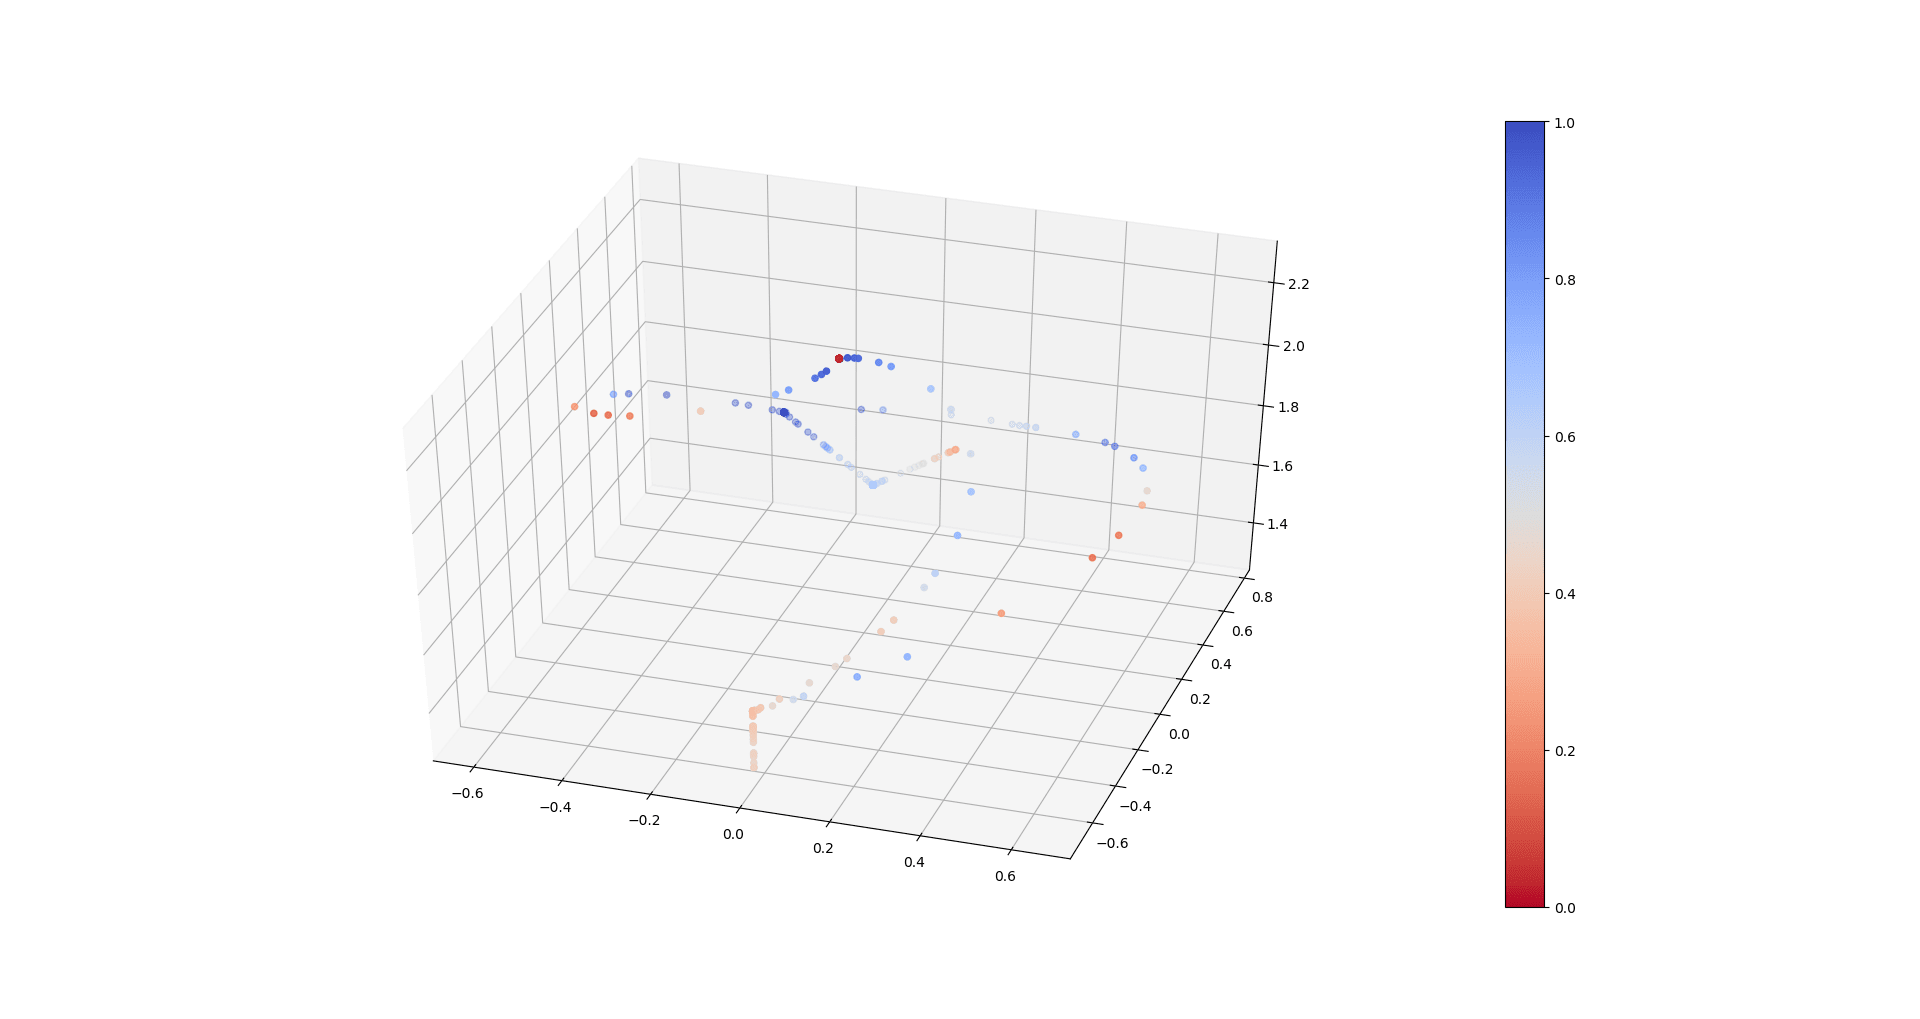
\includegraphics[width=10cm]{images/robot-planner1-manipulability-plot.png}\\
\caption{Plot the manipulability of the robot arm at sample points of the executed trajectory}
\end{figure}
\end{center}

The \ref{joint-limit-measure} equation calculates a joint limit measure which is multiplied with the manipulability measure and gives the dexterity measure.
From that equation we can conclude the following:
\begin{itemize}
\item If $q_i = q_{min}$ or $q_i = q_{max}$ then the exponential is equal to 1 which means that $\mathcal{L}_{q}$ and $\mathcal{D}$ are both 0, which means 
that the robot has \textbf{no dexterity at the boundary of the task space}.
\item If the value of $q_i$ is close to it's boundary value then the dexterity approches 0. The how mush close or far it is from the boundary (or in other words 
how fast the exponential term converges) depends on the parameter $\kappa$
\item The $q_{min}, q_{max}$ are calculated from the geometry of the task-space
\end{itemize}

For maximum dexterity at most points of a trajectory in a pivoting motion, the pivot sub-
taskspace (i.e. the space of all configurations of feasible pivot motions) must be fully within 
the robot’s whole reachable taskspace, otherwise only a small range of pivot movements will be 
feasible.